\chapter{Acoustic Perturbation Equations Solver}

\section{Synopsis}
The aim of APESolver is to predict aerodynamic sound generation. Through
the application of a splitting technique, the flow-induced acoustic field is
totally decoupled from the underlying incompressible hydrodynamic field. The
acoustic perturbation equations (APE-1/APE-4) proposed by Ewert and Shroeder are employed as
the governing equations of the acoustic field and they assure stable
aeroacoustic simulation due to the suppression of the term related to the
production of perturbed vorticity. These equations are similar to the linearised
perturbed compressible equations, but while in the original formulation the flow
decomposition is based on solenoidal vortical perturbations as well as
irrotational acoustic perturbations, in this case perturbations are assumed to
be exclusively of acoustic nature.
\begin{subequations}
    \begin{align*}
        \frac{\partial p'}{\partial t}
        + \frac{\partial \gamma \overline{p} u'_i}{\partial x_i}
        + \frac{\partial \overline{u}_i p'}{\partial x_i}
        &= \overline{c}^2 q_c
        \\
        \frac{\partial u'_i}{\partial t}
        + \frac{\partial \overline{u}_j u'_j}{\partial x_i}
        + \frac{\partial p' / \overline{\rho}}{\partial x_i}
        &= U_i
        \end{align*}
\end{subequations}
where $(\overline{u}_i,\overline{p}, \overline{\rho}, \overline{c}^2 = \gamma \overline{p} / \overline{\rho} )$ represents the base flow and $(u'_i,p')$ the perturbations.
$\overline{c}^2 q_c$ is the acoustic source term.

\section{Usage}
\begin{lstlisting}[style=BashInputStyle]
APESolver session.xml
\end{lstlisting}

\section{Session file configuration}

\subsection{Solver Info}
\begin{itemize}
\item \inltt{Eqtype} Specifies the equation to solve. This should be set to
\inltt{APE}.
\item \inltt{UpwindType} Specifies the numerical interface flux scheme.
Currently, only \inltt{APEUpwind} supported.
\end{itemize}

\subsection{Parameters}
\begin{itemize}
\item \inltt{Gamma}: Ratio of specific heats
\end{itemize}

\subsection{Functions}
\begin{itemize}
\item \inltt{BaseFlow} Baseflow $(\overline{u}_i, \overline{p}, \overline{\rho})$ defined by the variables \inltt{u0,v0,w0,p0,rho0}
\item \inltt{Source} Source term $\overline{c}^2 q_c$
\item \inltt{InitialConditions}
\end{itemize}


\section{Examples}
\subsection{Aeroacoustic Wave Propagation}
In this section we explain how to set up a simple simulation of aeroacoustics in
Nektar++. We will study the propagation of an acoustic wave in the simple case
where the base flow is $\overline{u}_i = 0, \, \overline{p}=p_{\infty}=10^6, \, \overline{\rho} = \rho_0 = 1.204$. The geometry consists
of $64$ quadrilateral elements, as shown in Fig.~\ref{f:apesolver:geometry}.

\begin{figure}
	\centering
	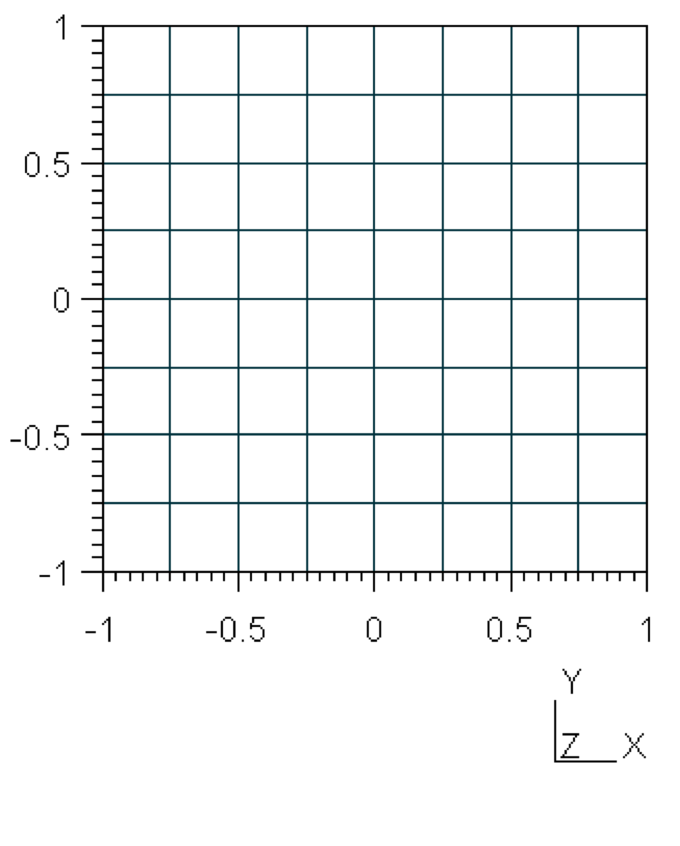
\includegraphics[width=0.5\linewidth]{img/APE_Geometry.png}
	\caption{Geometry used for the example case of modelling propagation of
	acoustic waves where $\overline{u}_i = 0, \, \overline{p}=p_{\infty}=10^6, \, \overline{\rho} = \rho_0 = 1.204$}
	\label{f:apesolver:geometry}
\end{figure}

\subsubsection{Input file}
We require a discontinuous Galerkin projection and use an explicit
fourth-order Runge-Kutta time integration scheme. We therefore set the following
solver information:
\begin{lstlisting}[style=XmlStyle]
<I PROPERTY="EQType" VALUE="APE"/> 
<I PROPERTY="Projection" VALUE="DisContinuous"/>
<I PROPERTY="TimeIntegrationMethod"  VALUE="ClassicalRungeKutta4"/>
<I PROPERTY="UpwindType"  VALUE="APEUpwind"/>
\end{lstlisting}

To maintain numerical stability we must use a small time-step. The total
simulation time is $150$ time units. Finally, we set the density, heat ratio and
ambient pressure.
\begin{lstlisting}[style=XMLStyle]
<P> TimeStep       = 0.00001             </P>
<P> NumSteps       = 150                 </P>
<P> FinTime        = TimeStep*NumSteps   </P>
<P> Rho0           = 1.204               </P> <!-- Incompressible density -->
<P> Gamma          = 1.4                 </P> <!-- Ratio of specific heats -->
<P> Pinfinity      = 100000              </P> <!-- Ambient pressure -->
\end{lstlisting}

Let us note that to solve efficiently this problem a discontinuous Garlerkin
approach was used. The
system is excited via the initial conditions putting a Gaussian pulse for pulse
fluctuations.  Finally, it is necessary to specify the base flow and the
eventual source terms using the following functions:

\begin{lstlisting}[style=XmlStyle]
<FUNCTION NAME="Baseflow"> 
    <E VAR="u0"   VALUE="0" />
    <E VAR="v0"   VALUE="0" />
    <E VAR="p0"   VALUE="Pinfinity" />
    <E VAR="rho0" VALUE="Rho0" />
</FUNCTION>

<FUNCTION NAME="Source"> 
    <E VAR="S"  VALUE="0" />
</FUNCTION>

<!-- Gaussian pulse located at the origin -->
<FUNCTION NAME="InitialConditions">
    <E VAR="p" VALUE="100*exp(-32*(((x)*(x))+((y)*(y))))" />
    <E VAR="u" VALUE="0" />
    <E VAR="v" VALUE="0" />
</FUNCTION>
\end{lstlisting}

\subsubsection{Running the code}
\begin{lstlisting}[style=BashInputStyle]
APESolver Test_pulse.xml
\end{lstlisting}

\subsubsection{Results}
Fig.~\ref{f:apesolver:results} shows the pressure profile at different
time steps, showing the acoustic propagation.

\begin{figure}
	\centering
	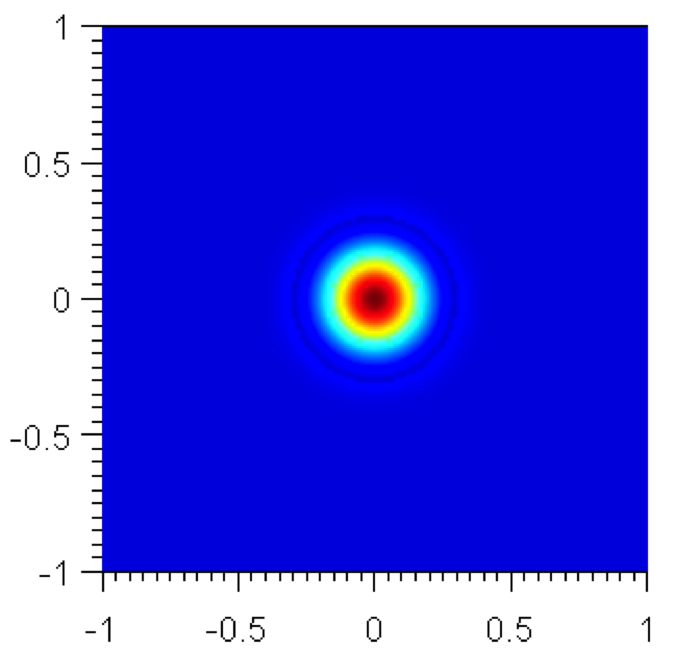
\includegraphics[width=0.3\linewidth]{img/Prop_1.png}
	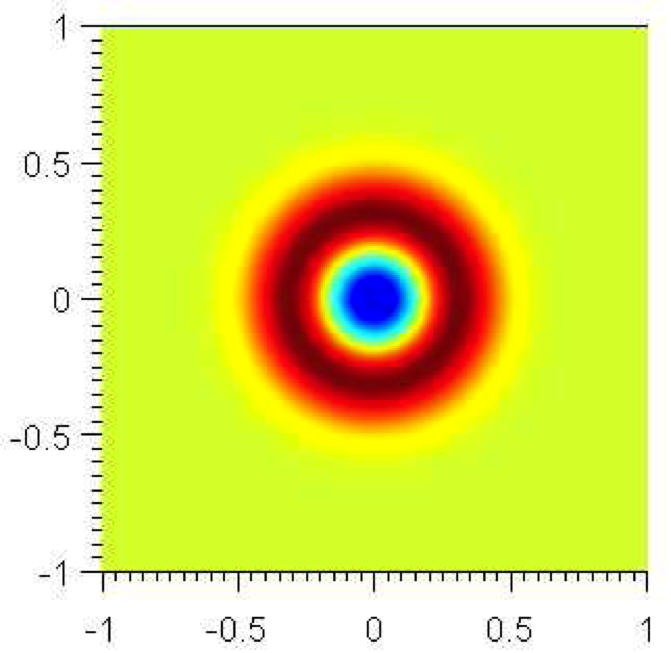
\includegraphics[width=0.3\linewidth]{img/Prop_2.png}
	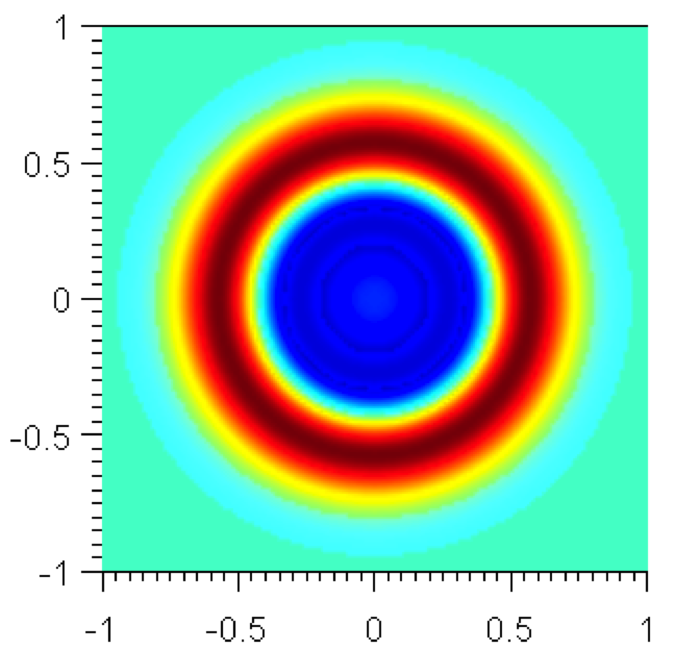
\includegraphics[width=0.3\linewidth]{img/Prop_3.png}
	\caption{}
	\label{f:apesolver:results}
\end{figure}

It is possible to show the profile of the pressure perturbations with respect to
the spatial coordinate. The pressure fluctuations, that are concentrated  in a
specific locations at the beginning (as specified by the initial conditions),
propagate with time and for sufficiently large time the decay is exponential as
predicted by literature \cite{DoFf83}.

\begin{figure}
	\centering
	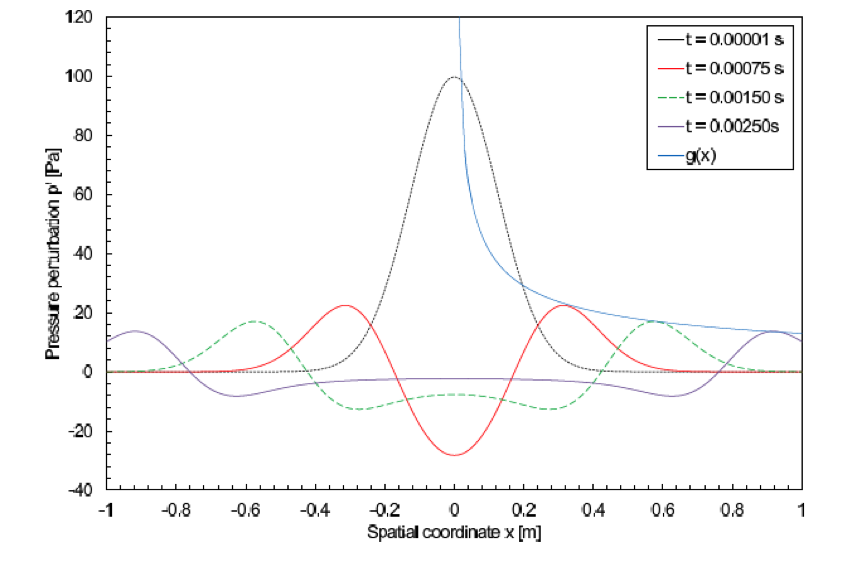
\includegraphics[width=0.7\linewidth]{img/prog_4.png}
	\caption{}
\end{figure}

